%!TEX program = lualatex
\documentclass[border=0mm,11pt]{standalone}
%\usepackage{color}
%\usepackage{tikz}
\usepackage[T1]{fontenc}
\usepackage[sc]{mathpazo}
\usepackage{tikz-feynman}
\usepackage{amsmath}
\tikzfeynmanset{compat=1.1.0}


\begin{document}

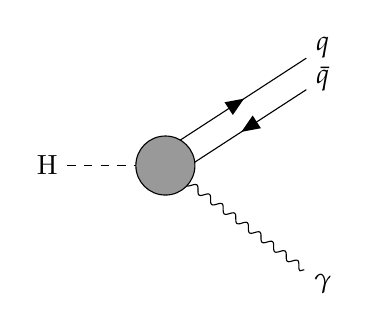
\begin{tikzpicture}[]
    \begin{feynman}[every blob={/tikz/fill=gray!80,/tikz/inner sep=0pt}]
    \vertex (h) {H};
    \vertex [right=of h, xshift=0.0cm, yshift=-0.0cm] (cent);
    \vertex [right=of h, xshift=2.0cm, yshift=1.5cm] (b) {$q$};
    \vertex [right=of h, xshift=2.0cm, yshift=1.1cm] (e) {$\bar{q}$};
    \vertex [right=of h, xshift=0.266666667cm, yshift=-0.2cm] (middle);
    \vertex [right=of h, xshift=2.0cm, yshift=-1.5cm] (f) {$\gamma$}; 
    \vertex [right=of h, xshift=0.0cm, yshift=0.2cm] (cent_s1);
    \vertex [right=of h, xshift=0.0cm, yshift=-0.2cm] (cent_s2);
    
    \diagram* {
    (h) -- [scalar] (cent),
    (b) -- [with reversed arrow=0.55] (cent_s1),
    (e) -- [with arrow=0.40] (cent_s2),
    (cent) -- [photon] (f),
    };
    \node [blob] at (cent) {};
    \end{feynman}
\end{tikzpicture}

\end{document}